% !!!!!!!!!!!!!!!!!!!!!!!!!!!!!!!!!!!!!!!!!!!!!!!!!!!!!!!!!!!!!!!!!!!!!!!!!!!!
%                                                                            !
% Adapt this file so that you can use it for your thesis					 !
%                                                                            !
% !!!!!!!!!!!!!!!!!!!!!!!!!!!!!!!!!!!!!!!!!!!!!!!!!!!!!!!!!!!!!!!!!!!!!!!!!!!!


\documentclass{micro-econ-thesis}
\usepackage{graphicx}
\usepackage{setspace}
\usepackage{float}
\usepackage[utf8]{inputenc} % depends on the font encoding that you are using

% For formatting of your bibliography, please use the following package with options 
\usepackage[style=authoryear]{biblatex}
\usepackage{gensymb}

\addbibresource{bibliography.bib} % add a bib-reference file

\begin{document}
% ----------------------------------------------------------------------------
% Details for the titlepage
% ----------------------------------------------------------------------------
\thesisTitle{Develeopment of Analysis Techniques for dynamic magnetic resonance imaging}
\thesisType{Master Thesis} % 'Master Thesis' or 'Seminar Paper'
\thesisAuthor{Aayush Nepal}
\thesisMail{aayush.nepal@uni-jena.de}
\thesisGrade{Master of Science in Medical Photonics} % leave empty for seminar papers
\thesisTutora{Prof. Dr. rer. nat. med. habil. Jürgen Reichenbach}
\thesisTutorb{Dr. rer. nat. Martin Krämer}
\thesisMatrikel{198683}
\thesisAddress{Schützenggase 2\\[.5ex]
								99423 Weimar}
\thesisDate{\today}
% In case of external supervisor
\thesisCompany{}

% Print titlepage
\thesisMakeTitle

% ----------------------------------------------------------------------------
% Abstract
% ----------------------------------------------------------------------------
\cleardoublepage
\pagenumbering{roman}
\pagestyle{plain}
%\thispagestyle{empty}
\subsection*{Abstract}
Short summary of your thesis (max. 250 words) \ldots

\clearpage
\subsection*{Acknowledgements}
If you want to thank anyone (optional) \ldots

% ----------------------------------------------------------------------------
% Table of contents
% ----------------------------------------------------------------------------
\cleardoublepage
%\thispagestyle{empty}
\tableofcontents

% ----------------------------------------------------------------------------
% List of figures/tables
% ----------------------------------------------------------------------------
\cleardoublepage
\phantomsection
\addcontentsline{toc}{section}{List of Figures}
\listoffigures
% --------------------------
\cleardoublepage
\phantomsection
\addcontentsline{toc}{section}{List of Tables}
\listoftables
% --------------------------

\cleardoublepage
\phantomsection
\addcontentsline{toc}{section}{List of Acronyms}
\section*{List of Acronyms}
\begin{tabular}{@{}ll}
FSU Jena & Friedrich-Schiller-Universität Jena\\
\end{tabular}

% --------------------------

% ----------------------------------------------------------------------------
% Contents
% ----------------------------------------------------------------------------
\cleardoublepage
\pagestyle{headings}
\pagenumbering{arabic}
\setcounter{page}{1}
% Contents
\onehalfspacing % for linespacing 1.5, you can turn it off with \singlespacing, e.g. for quotes or tables with multiline cells


\section{Introduction}
\label{sec:intro}


\subsection{The Knee }
The knee, a pivotal structure in the human body, plays an essential role in locomotion. Additionally, it functions to control the center of body mass and posture in the activities of daily living by facilitating a wide range of movements. As such, the knee's health and integrity are vital for overall quality of life, influencing everything from basic mobility to participation in complex sports. In a comprehensive survey across 15 European countries and Israel, it was found that knee pain was the third most commonly reported location of chronic pain, highlighting the significant concern it poses to public health \parencite{breivik_survey_2006}. Furthermore, arthritis/osteoarthritis (OA) was identified as the most common cause of this pain. 

And this situation has not improved with time. In Germany for instance, a recent retrospective study has found that the number of patients with OA is steadily rising \parencite{obermuller_epidemiology_2024}. 
Part of the reason knee-related issues are so prevalent and impactful is the inherent complexity of the knee joint itself. As a hub of various anatomical structures working in unison, the knee supports a range of movements and bears significant loads, making it susceptible to a variety of injuries and conditions.
Understanding the anatomy of the knee is the first step in tackling this problem. 

\textbf{Anatomy and Function}

The knee joint is the largest and the most superficial synovial joint in the body. \parencite{dalley_moores_2023}. 
It comprises three primary articulations:two femorotibial articulations (see Figure \ref{fig:rightkneeplate519}) and one femoropatellar articulation. These articulations, illustrated in figures \ref{fig:rightkneeplate519} and \ref{fig:patellarsurface}, are defined by their complexity and incongruence, features that are crucial for the joint's biomechanical performance. 
 
\begin{figure}[H]
	\centering
	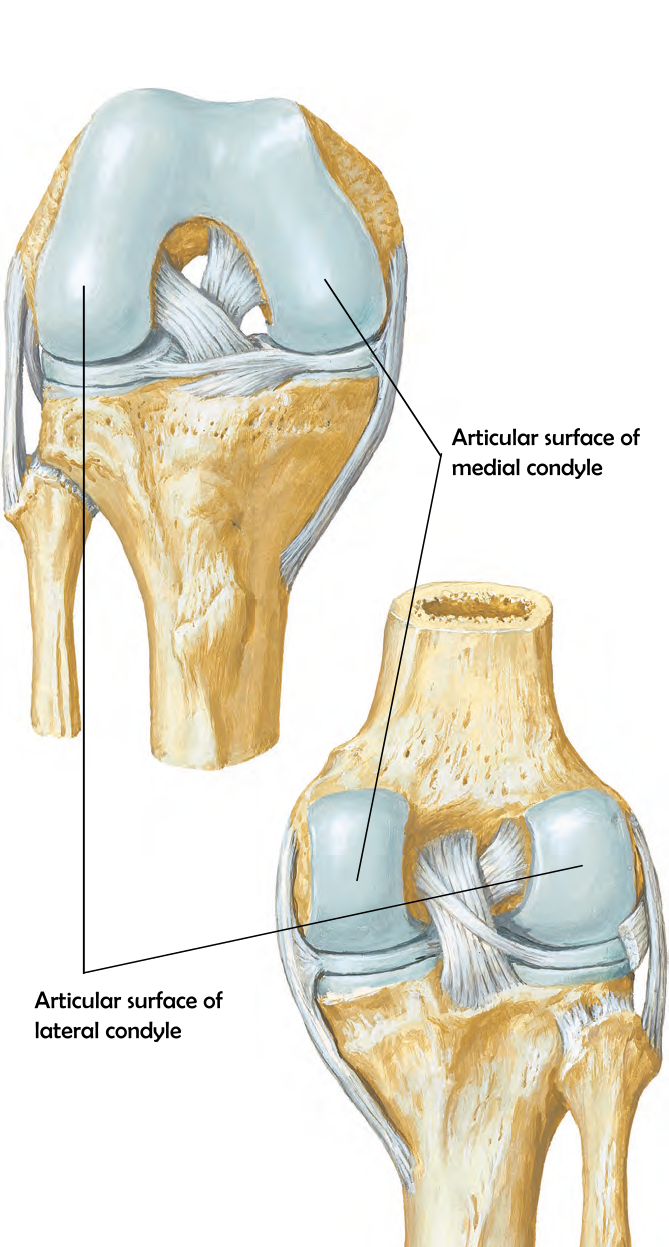
\includegraphics[width=0.7\linewidth]{right_knee_labeled}
	\caption{Anterior (flexed,top) and posterior (extended, bottom) view of the right knee with their articular surfaces labeled. \parencite[p.519]{netter_519_2023}}
	\label{fig:rightkneeplate519}
\end{figure}

\begin{figure} [H]
	\centering
	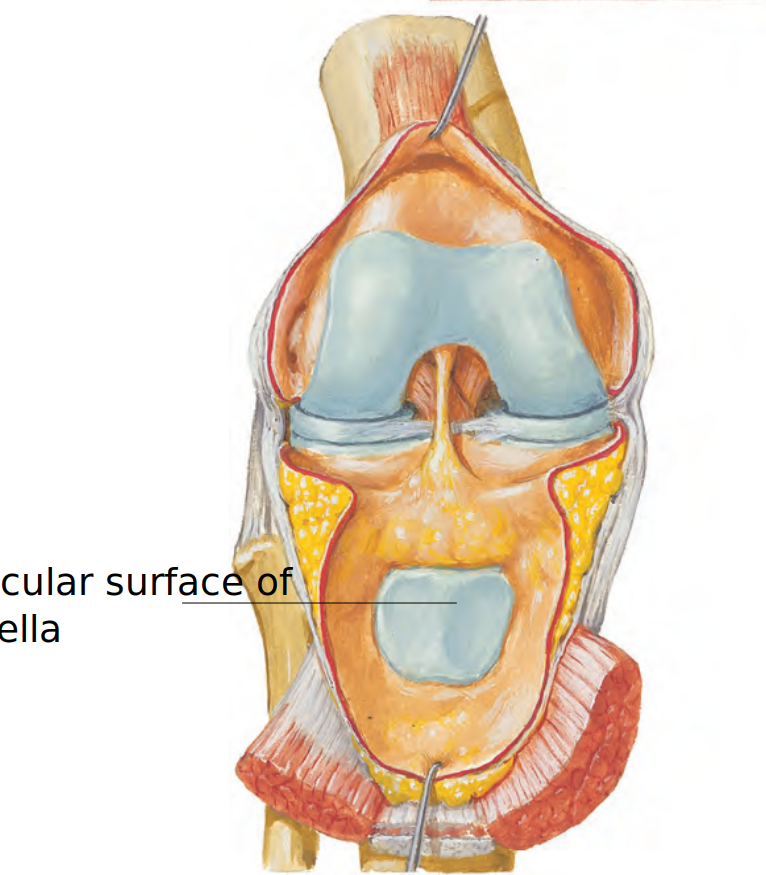
\includegraphics[width=0.7\linewidth]{patellar_surface}
	\caption[patellar surface]{Right joint opened, knee slightly in flexion, with the patellar articulation labelled. \parencite[p.517]{netter_519_2023}}
	\label{fig:patellarsurface}
\end{figure}

This design allows the knee to manage a wide array of movements and bear significant loads. Figure \ref{fig:sixdegrees} illustrates the knee's capacity for multidimensional movement, highlighting the joint's sophisticated structural design that enables this versatility. However, this inherent design also renders the knee vulnerable to a range of forces \parencite{standring_grays_2021}.

Such mechanical forces, influenced by activities and body mass index (BMI), are significant causes of OA and represent one of the most modifiable risk factors \parencite{heidari_knee_2011}. Furthermore, abnormal joint loading is considered a key mechanical driver of osteochondral changes thought to contribute to the initiation and progression of knee OA \parencite{coburn_immediate_2023}.

\begin{figure}[H]
	\centering
	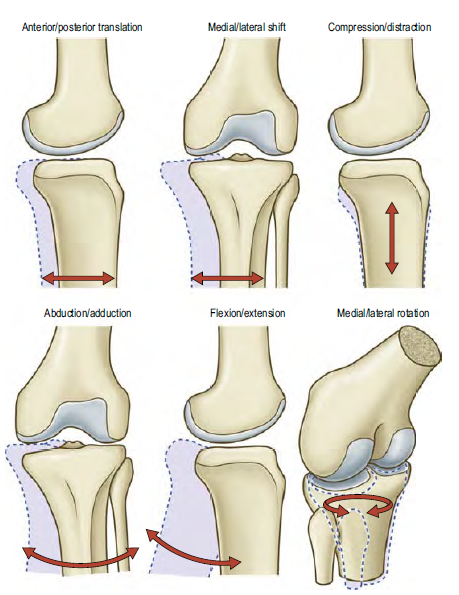
\includegraphics[width=0.7\linewidth]{six_degrees}
	\caption{The knee joint motion in three dimensions, described using six independent variables (degrees of freedom) \parencite[p.~1412]{standring_grays_2021}.}
	\label{fig:sixdegrees}
\end{figure}

The relationship between biomechanical stresses and knee health highlights the need for diagnostic tools that fulfill two key criteria: they must capture the knee's dynamic behavior during motion and assess the joint under varying loads. Dynamic magnetic resonance imaging (MRI) excels in meeting these requirements as one of the most advanced imaging modalities.

\subsection{Dynamic MRI}
In a broad sense, dynamic MRI is an umbrella term encompassing various MRI techniques designed to capture and visualize physiological processes and motion over time. This dynamic aspect of MRI is crucial when studying systems or structures where motion is inherent, such as blood flow, tissue perfusion, or cardiac movement. For the purposes of this project, the focus of "dynamic MRI" narrows down to capturing the bulk movement of the knee joint undergoing active flexion extension cycles inside the scanner. Compared to traditional static MRI scans, which are highly susceptible to motion artifacts compared to other imaging modalities \parencite{zaitsev_motion_2015}, dynamic MRI techniques not only accommodates motion, but can even leverage it to offer comprehensive insights into the functional and biomechanical properties of the concerned structures.  Among these techniques, CINE imaging, particularly renowned in cardiac MRI, is considered the gold standard for evaluating cardiac function \parencite{menchon-lara_reconstruction_2019}. This high regard in cardiac MRI illustrates the method's precision and adaptability, traits we leverage for knee imaging.

\textbf{CINE imaging}

CINE is derived from the word cinematography, to create a movie. In the context of dynamic knee MRI, this technique can be used to reconstruct a "movie" of a single flexion-extension cylce. This is done by stiching together many partial datasets from multiple cylces. The full flexion-extension cycle is divided into distinct stages where each stage corresponds to a particular flexion angle. The full
" 
Dynamic cardiac MRI is conventionally performed with a
technique known as CINE,13 which takes its name from cine-
matography. In brief, a “movie” of a single beating heart cycle
is reconstructed by literally stitching together numerous par-
tial datasets from many heartbeats—typically 15–18, more if
multiple slices are acquired. Because data acquisition is too
slow to collect all data in a single heartbeat, acquisition is seg-
mented over several heartbeats. Specifically, the cardiac cycle
is divided into many phases (or timepoints), and the fully
sampled k-space for each phase is divided into multiple seg-
ments (Fig. 1). Once all segments for all cardiac phases are
acquired, the data are temporally reordered and converted to
the image domain to produce the impression of a continu-
ously acquired time series. One can readily appreciate that
this technique does not provide real-time dynamics and works
robustly only if cardiac cycles are sufficiently similar.

" 
\parencite{curtis_primer_2022}
 
To achieve this, we require not only an imaging sequence and reconstruction technique, but also a MR safe knee loading device. They are described in the section below. 

\subsection{Foundational Work}
This project builds upon two distinct works: the construction of the MRI knee loading device \parencite{brisson_novel_2022}  and the development of the imaging sequence used for capturing and reconstructing the data. \parencite{aleksiev_high-resolution_2022}

\textbf{High resolution CINE imaging}

This imaging technique presents a significant advancement in capturing active knee motion. 
It combines continuously acquired radial golden-angle MRI data with angular sensor information to retrospectively reconstruct CINE images of the knee, allowing the acquisition of high-resolution 2D images during knee flexion and extension. 






\textbf{Knee loading device }

\subsection{Research Necessity}
Discuss the necessity for further analysis of the acquired images, emphasizing the gap between data collection and data interpretation within the current literature.

Clearly state the objectives of your research, focusing on the development of new analytical techniques to interpret the existing dynamic MRI data.

Explain the expected contributions of your research to the field, including the potential implications for biomechanical understanding and clinical applications.

\subsection{Thesis Structure}
Structure of the thesis is as follows: 


\section{Methodology}
\label{sec:second}
some text 
\subsection{Data Collection Methods}
\subsubsection{The Device}
A novel MRI-compatible device was integrated into the MRI scanner setup to facilitate guided knee motion in patients \parencite{brisson_novel_2022}. This device allowed for a range of motion of approximately 30 degrees, enabling subjects to perform knee flexion and extension cycles under both loaded and unloaded conditions. For loading, the device was equipped with compartments for weight plates \underline{(maybe picture here?)} and sandbags, providing a physiological load of 10 to 12 kilograms. 


Central to this device's functionality is an optical fiber position sensor \underline{actual citation needed?}(MR338-Y10C10, Micronor, 155 Camarillo, CA, USA), which precisely  which measures the ab­
solute angle from 0{\degree}\,to 360\degree \, with a resolution of 0.025\degree. This measurement capability is critical for synchronizing the knee's movement with MRI data reconstruction. To enhance signal acquisition and the clarity of imaging, two flexible coils \underline{(cite the coils here, perhaps also show a picture)} were positioned at key anatomical locations: one at the distal femur and another at the proximal tibia, as specified in the MRI protocol. \underline{perhaps show a picture outside the scanner of the patient wearing it? }

\subsubsection{Procedure Details}
***MRI measurements were performed on four healthy volunteers (aged between 28 and 37 years, body mass between 55 and 90 kg) using a clinical 3 T Siemens Prisma fit scanner. Volunteers had no known musculoskeletal conditions and gave written informed consent in accordance with the guidelines set out by the institutional ethics committee.*** \underline{from device paper} For all of these subjects, the left leg was used. 

The thigh is secured on a wedge positioner, and the lower leg is attached to an ankle rest, just above the malleoli, using Velcro straps to minimize lateral movement. Once positioned at the scanner's isocenter, the volunteer then engages in a controlled exercise, following a metronome set at 60 beats per minute. This pace dictates a four-beat flexion to extension cycle, where the leg is flexed at the first beat and fully extended by the fourth. This exercise is performed for approximately 2 minutes throughout the duration of the scan, totaling between 100 to 120 repetitions. Initially conducted under a loaded condition with weights, the process is repeated without the added resistance to compare both states.

\subsubsection{Sequence Parameters and Reconstruction}


\subsection{Data Analysis}
All the analysis and data visualization were done using the python programming language (v3.11.5). To begin, the data in nifti (Neuroimaging Informatics Technology Initiative) format is loaded using nibabel (v5.1.0) library. It is then visualized using napari(v0.4.18), a multi-dimensional interactive image viewer in Python. 
\subsubsection{Segmentation}
Step 1: Edge Detection Using the Canny Algorithm

The Canny filter \parencite{canny_computational_1986}, as implemented in the scikit-image's feature library (v0.21.0), was employed to apply an edge filter to the images. Various parameters of the Canny algorithm were adjusted, including edge thresholds and Gaussian blur, to optimize edge detection. Subsequently, the scikit-image's morphology library was utilized to remove small elements from the binary image. The image was then skeletonized to a one-pixel width, retaining only long and consistent edges. The final selection of the desired edge was accomplished using scipy's label algorithm (v1.11.3).

\subsection{Validity and Reliability}
Validation Methods: Detail the steps taken to validate the segmentation techniques and the biomechanical parameters you derived.
Reliability Measures: Describe any repeat analyses or cross-verifications done to ensure the consistency and reliability of your results.

\section{Results}
\label{sec:yetanother}

\subsection{Segmentation}
\label{subsec:last}
some text 

\subsection{Parameter Extraction}
some text 

\section{Discussion}
\subsection{Technique Evaluation}
Assess the effectiveness and accuracy of your segmentation techniques. 
\subsection{Biomechanical Insights}
Discuss the biomechanical parameters obtained and their implications for understanding knee movement. 
\subsection{Comparison with Existing Methods}
Compare your results with current analysis techniques. 
 

\section{Conclusion}
\subsection{Summary of Contributions}
Recap the novel analysis techniques developed and their significance. 
\subsection{Limitations and Challenges}
Discuss any limitations encountered and the challenges in the analysis process 
\subsection{Future Work}
Suggest potential improvements and future directions for research

% ----------------------------------------------------------------------------
% Bibliography
% ----------------------------------------------------------------------------
\cleardoublepage
\phantomsection
\addcontentsline{toc}{section}{\refname} % to add Bibliography to toc
\printbibliography

% --------------------------
\cleardoublepage
\begin{appendix}
\section{Appendix}
If needed for supplementary material, such as detailed description of data collection, tables, or figures.

\end{appendix}

% ----------------------------------------------------------------------------
% Statutory declaration
% ----------------------------------------------------------------------------
\makeThesisDeclaration

\end{document}

